\documentclass[10pt,twocolumn,letterpaper]{article}

\usepackage{cvpr}
\usepackage{times}
\usepackage{epsfig}
\usepackage{graphicx}
\usepackage{amsmath}
\usepackage{amssymb}
\usepackage[
backend=biber,
%style=numeric,
citestyle=numeric 
]{biblatex}
\addbibresource{egbib.bib}

% Include other packages here, before hyperref.

% If you comment hyperref and then uncomment it, you should delete
% egpaper.aux before re-running latex.  (Or just hit 'q' on the first latex
% run, let it finish, and you should be clear).
\usepackage[breaklinks=true,bookmarks=false]{hyperref}

\cvprfinalcopy % *** Uncomment this line for the final submission

\def\cvprPaperID{****} % *** Enter the CVPR Paper ID here
\def\httilde{\mbox{\tt\raisebox{-.5ex}{\symbol{126}}}}

% Pages are numbered in submission mode, and unnumbered in camera-ready
%\ifcvprfinal\pagestyle{empty}\fi
\setcounter{page}{1}
\begin{document}

%%%%%%%%% TITLE
\title{Crowd counting on fixed camera images}

\author{Pierpaolo D'Odorico\\
{\tt\small pierpaolo.dodorico@studenti.unipd.it}
\and
Massimiliano Conte\\
{\tt\small massimiliano.conte@studenti.unipd.it}
}


\maketitle
%\thispagestyle{empty}
\begin{abstract}



In this work we compared different computer vision tecniques in order to estimate the number of people in a frame. The counting is performed on images captured from a fixed camera placed in a shopping mall. Some applications of this kind of counting on a static view are security and safety tasks, estimating the number of visitors on a mall for a/b testing purpose, planning spaces and services or verify compliance with covid-19 social distancing.

\end{abstract}

%%%%%%%%% BODY TEXT
\section{Introduction}

The crowd counting problem received a lot of attention in recent years, due to its direct connection with crowd control and public safety. For this reason many techniques were recently proposed.
Our idea is to compare two main tecniques in this fixed camera setting, one that is fast to implement and the other one more challenging, in order to verify if it is worth it to spend time for a more sophisticated solution. The first approach is to direcly estimate the number of people performing regression with a convolutional neural network, such as the VGG16 network \cite{simonyan2014very}.  This very deep network was proposed by K. Simonyan and A. Zisserman from the University of Oxford and it was submitted to ImageNet challenge in 2014. The second approach deals with density maps. Those are useful in real life applications since the same number of people could have completely different crowd distributions. (as shown in Fig. 1). After implementing the two approaches on our problem we found that...


%------------------------------------------------------------------------
\section{Related work}

We based our project on informations contained in different papers about computer vision tasks and crowd counting. The first one is related to VGG16, the network we fine tuned for dealing with our people counting problem \cite{simonyan2014very}. In this paper the authors investigate the effect of the convolutional network depth on its accuracy in the
large-scale image recognition setting. In this convolutional neural networks they use very small (3x3) convolution filters, which shows that a significant improvement on the prior state of the art configurations. They also pushed the depth to 16-19 weight layers (Fig.\ref{fig:vgg16}). Those small convolutional filters can be useful in our application for finding people in images. Fine tuning the final layers and adding a regression one at the final part of the network, we hope that VGG16 model will achieve a good performance. 

\begin{figure}[h!]
  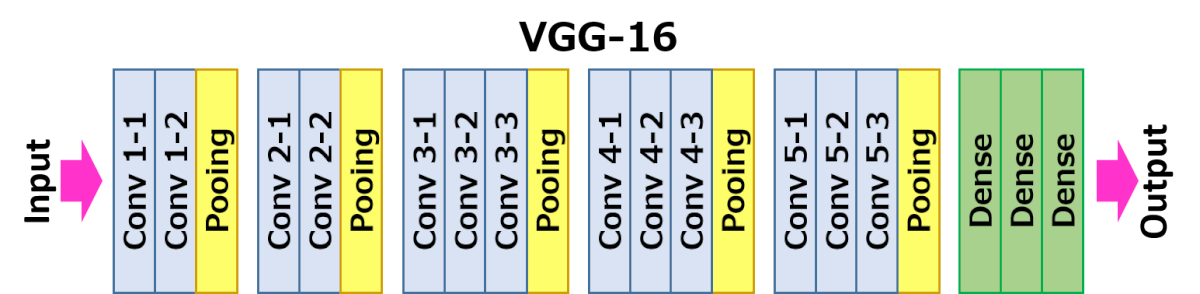
\includegraphics[width=\linewidth]{pics/vgg16.png}
  \caption{VGG16 deep CNN structure}
  \label{fig:vgg16}
\end{figure}

We relate also to two papers about density map crowd counting approach. In the first one \cite{zhang2016single} authors introduced a new large-scale crowd dataset named Shanghaitech. It contains nearly 1,200 images with around 330,000 accurately labeled heads. They also used Multi-column CNN for density map estimation (Fig.\ref{fig:densitymap}). We also relate to a more recent paper that simplifies the convolutional neural network of the previous work and achieves better results. This second paper about density map crowd couting approach \cite{li2018csrnet} uses a CSRNet architecture for capturing high-level features with
larger receptive fields and generating high-quality density maps without expanding network complexity. 

\begin{figure}[h!]
  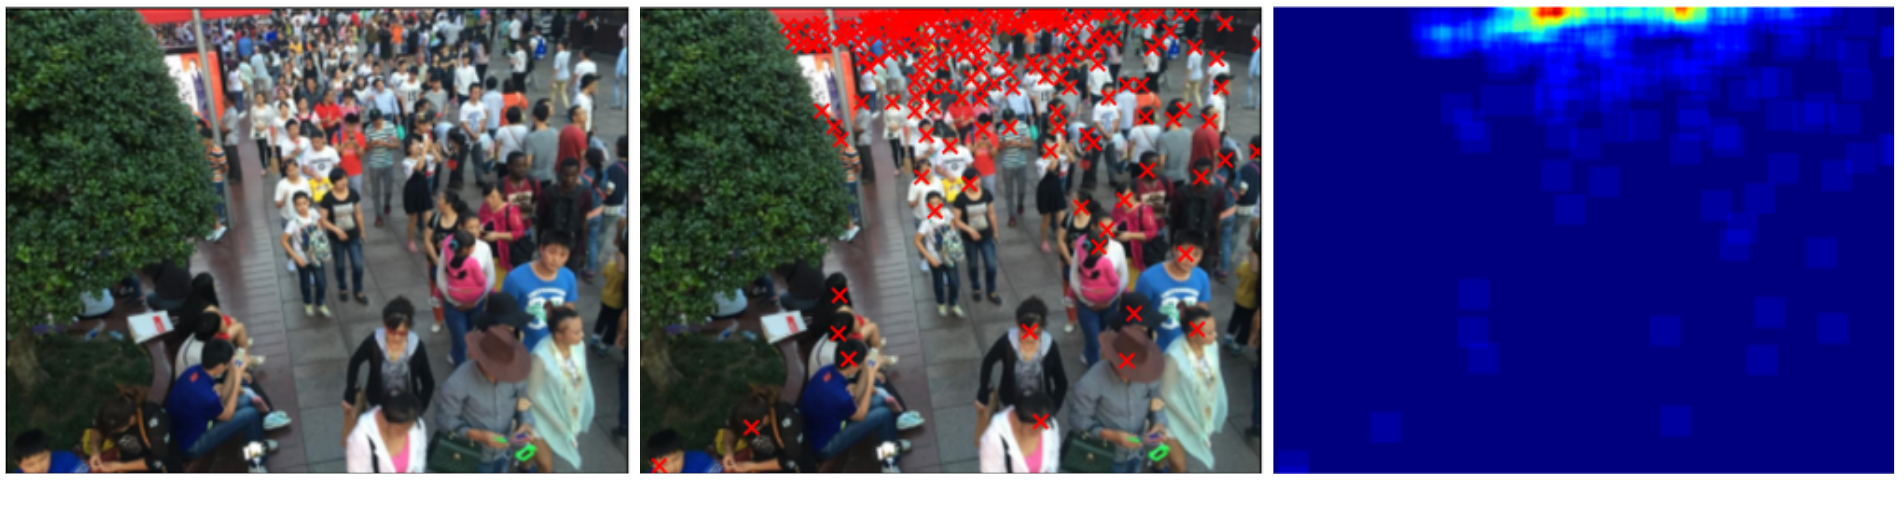
\includegraphics[width=\linewidth]{pics/densitymapapproach.png}
  \caption{Density map approach}
  \label{fig:densitymap}
\end{figure}



%------------------------------------------------------------------------
\section{Dataset}






%{\small
%\bibliographystyle{ieee_fullname}
%\bibliography{egbib}
%}

\end{document}
